\subsection{Scheduling robustness}
\label{sec:scheduling-protocol}
The default scheduling contrast raises a specific question: how much does it depend on the requests exposed to the controller? Earlier controller sweeps changed flat-replay placement; they do not answer this scheduling question. The final sensitivity matrix therefore compares all three schedules on BFS placement, using the ten reference splits and both footprints.

Six conditions change one assumption at a time. Three set the outstanding-transaction limit to 16, 32 or 128, retaining the 32-entry controller read buffer. Two split each candidate-vector phase into consecutive batches of at most two or eight vectors, draining each batch before the next starts. The last uses the previously evaluated alternative address mapper. All other settings match the default bounded model. This adds 360 replays; the 64-outstanding, full-phase default reuses the earlier evidence. The design was fixed before inspecting these timings, and every condition remains in the results.

\begin{figure}[htbp]\centering
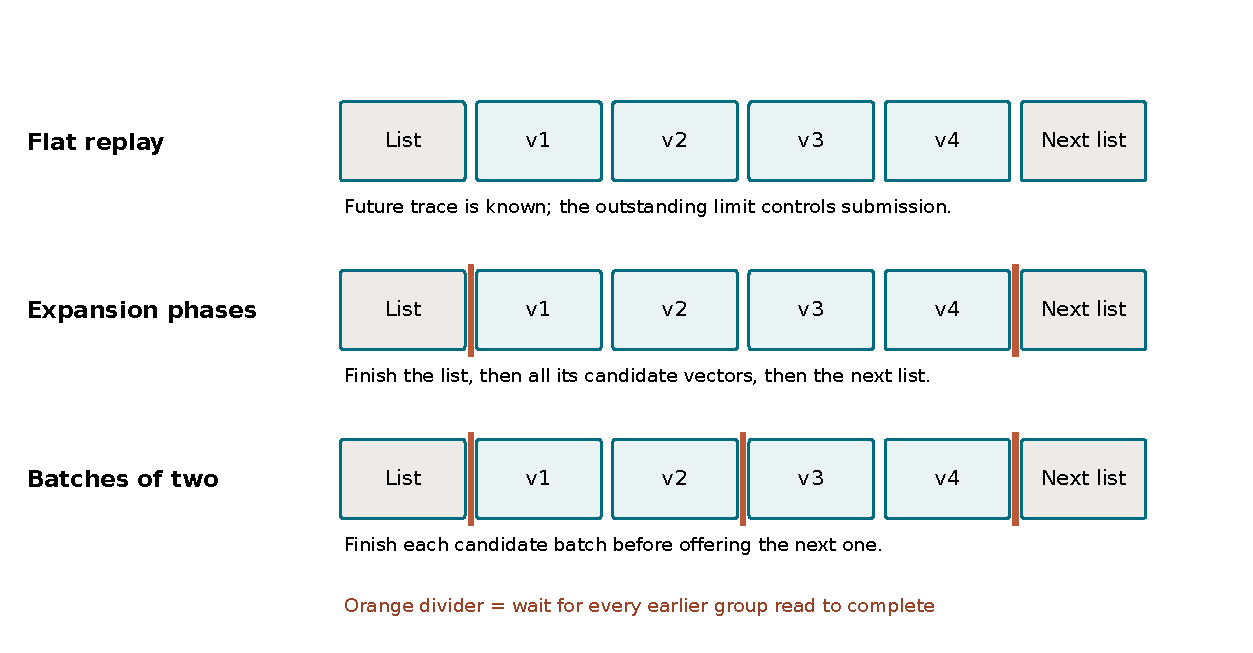
\includegraphics[width=\textwidth]{generated/replay_models.pdf}
\caption[What the replay boundaries mean]{The same illustrative logical sequence under three availability models. Orange dividers require completion of the preceding group. Vector reads inside a group may overlap subject to controller and outstanding limits. Horizontal position denotes request order, not elapsed time. All modes omit computation and integration costs.}\label{fig:replay-models}
\end{figure}

Figure~\ref{fig:replay-models} separates candidate batching from a transaction limit. A batch bounds the vectors whose chunks are offered before a drain; the outstanding limit bounds accepted reads that have not completed. A batch is not a rolling residency limit, and its extra drains can prevent overlap that a different implementation would exploit. Each schedule is compared with original order under exactly the same boundaries. Original-query service includes every inter-batch gap.

The emitter reproduces the previous flat BFS trace hashes before changing order, checks every batch's transaction multiset and retains the parent expansion of each batch. A one-vector batch supplies an exact sanity check: original order, sorting and round-robin produce identical streams. The retained evidence includes losslessly compressed phase timings, source/trace hashes, matched read counts and the complete named matrix. Pairing and confidence intervals follow Section~\ref{sec:paired}; reused queries do not turn this sensitivity study into independent confirmation. Graph-construction variation remains a separate experiment at default scheduling settings.
